\documentclass[aspectratio=169]{beamer}
\usetheme{Madrid}
\usecolortheme{beaver}
\usepackage[utf8]{inputenc}
\usepackage[T1]{fontenc}
\usepackage{tikz}
\usepackage{amssymb}
\usepackage{graphicx}
\setbeamertemplate{navigation symbols}{}
\setbeamercolor{title}{fg=white,bg=cyan!60!black}
\setbeamercolor{frametitle}{fg=white,bg=cyan!50!black}
\setbeamercolor{block title}{bg=cyan!15,fg=black}
\setbeamercolor{block body}{bg=cyan!5,fg=black}

\title{G3 — Decisions}
\subtitle{Touching? Score > 10? Out of bounds?}
\author{ByteForge --- Grade 7 --- Game Maker --- Week Overview}
\date{}

\begin{document}

\begin{frame}
    \titlepage
\end{frame}

\begin{frame}{This Week's Plan}
    \begin{itemize}
        \item Lesson 1: Traffic Light
        \item Lesson 2: Big or Small
        \item Lesson 3: Danger Zone
        \item[$\bigstar$] BOSS --- Dodge at the Edges (\texttt{lessonBoss.tex})
    \end{itemize}
\end{frame}

\begin{frame}{Real-World Example}
    \Large
    A real traffic light's three states (red/amber/green) is literally an if/else-if/else chain in the controller software — same three-way branch this chapter teaches. Minecraft redstone comparators/repeaters build these same IF-style circuits entirely out of blocks, no typed code at all.
\end{frame}


\begin{frame}{Image}
    \begin{center}
    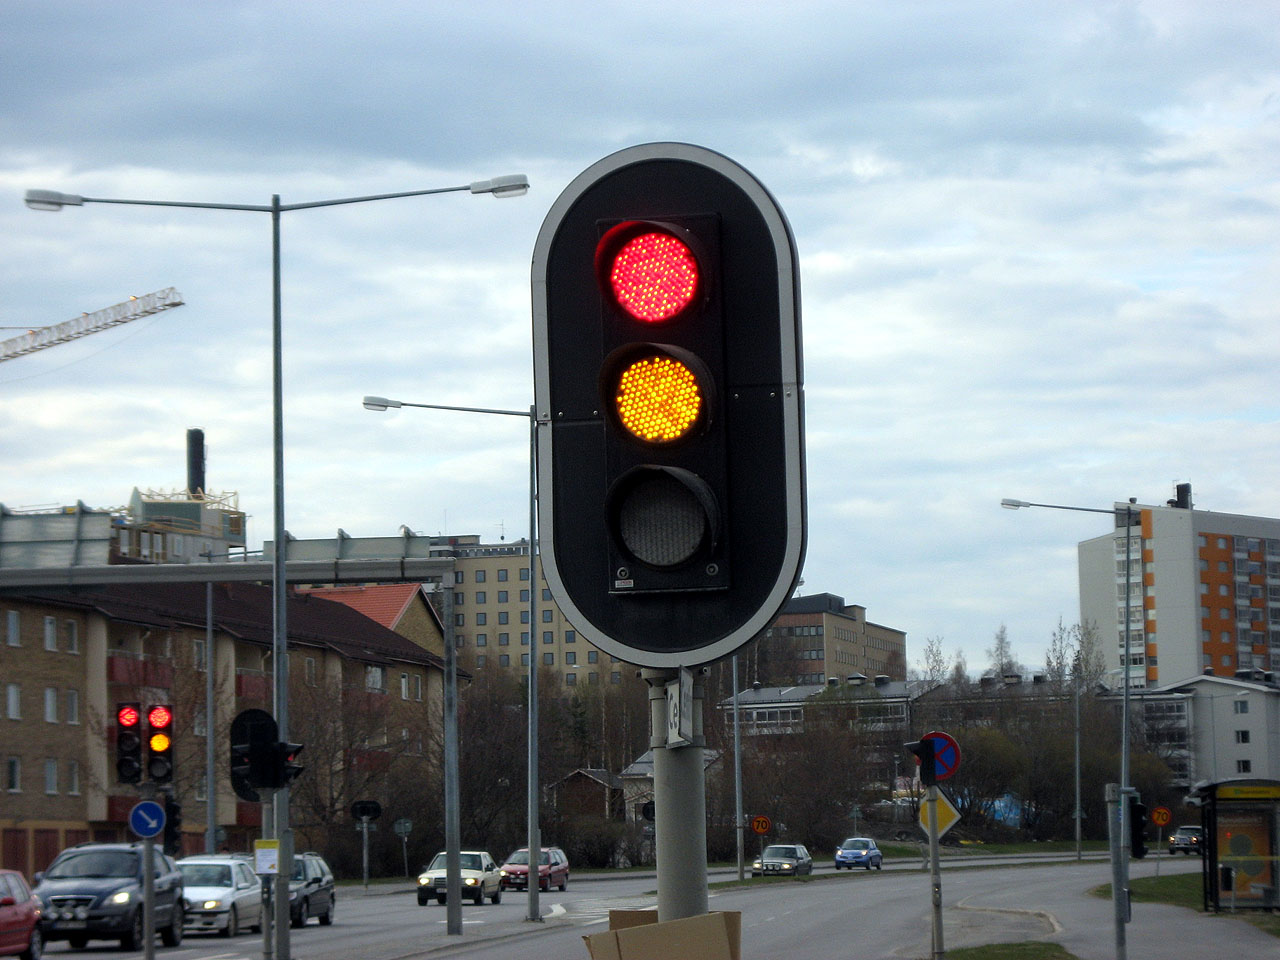
\includegraphics[width=0.55\textwidth]{../images/traffic.jpg}

    \small LED traffic lights, public domain (PD-self), via Wikimedia Commons
    \end{center}
\end{frame}

\begin{frame}{Let Them Discover}
    \Large
    Find a real rule with a fuzzy boundary (is a "tall" person over 180cm? over 175cm?). Where would YOU draw the line, and would someone exactly on that line be included or not? This is exactly the off-by-one problem in code.
\end{frame}

\begin{frame}{Files in This Folder}
    \small
    \begin{itemize}
        \item \texttt{lesson1.tex} --- Traffic Light
        \item \texttt{lesson2.tex} --- Big or Small
        \item \texttt{lesson3.tex} --- Danger Zone
        \item \texttt{lessonBoss.tex} --- BOSS: Dodge at the Edges
    \end{itemize}
    \vspace{0.5em}
    \normalsize Each lesson file is its own short deck --- open the one for
    the specific day you're teaching, not this whole overview.
\end{frame}

\end{document}
